\documentclass[graphics]{beamer}

\usepackage{graphicx}
\usepackage{verbatim}
\usepackage{wrapfig}
\useoutertheme{shadow}
%\usecolortheme{orchid}
\usecolortheme{seahorse}


% math commands
\newcommand{\be}{\begin{eqnarray}}
\newcommand{\ee}{\end{eqnarray}}
\newcommand{\beq}{\begin{equation}}
\newcommand{\eeq}{\end{equation}}
\def\simless{\mathbin{\lower 3pt\hbox
      {$\rlap{\raise 5pt\hbox{$\char'074$}}\mathchar"7218$}}}
\def\simgreat{\mathbin{\lower 3pt\hbox
      {$\rlap{\raise 5pt\hbox{$\char'076$}}\mathchar"7218$}}} %> or of order

% variables

\def\toonscale{0.45}
\def\mboxy#1{\mbox{\small #1}}


\begin{comment}
\AtBeginSection[]{
  \frame{
    \frametitle{Outline}
    \tableofcontents[currentsection]
  }
}
\end{comment}

\title{Fast Radio Bursts Overview
}
%\subtitle{interim update}
\author[U. Pen]{Ue-Li Pen and collaborators
}
\date{June 24, 2024}


\begin{document}

%\section*{Introduction}
\section{Lenses}

\begin{comment}
  \subsection{Outline}

  \frame{
    \frametitle{Outline}
    \tableofcontents
  }
\end{comment}

\frame{\maketitle}


  \frame{
    \frametitle{Fast Radio Bursts}
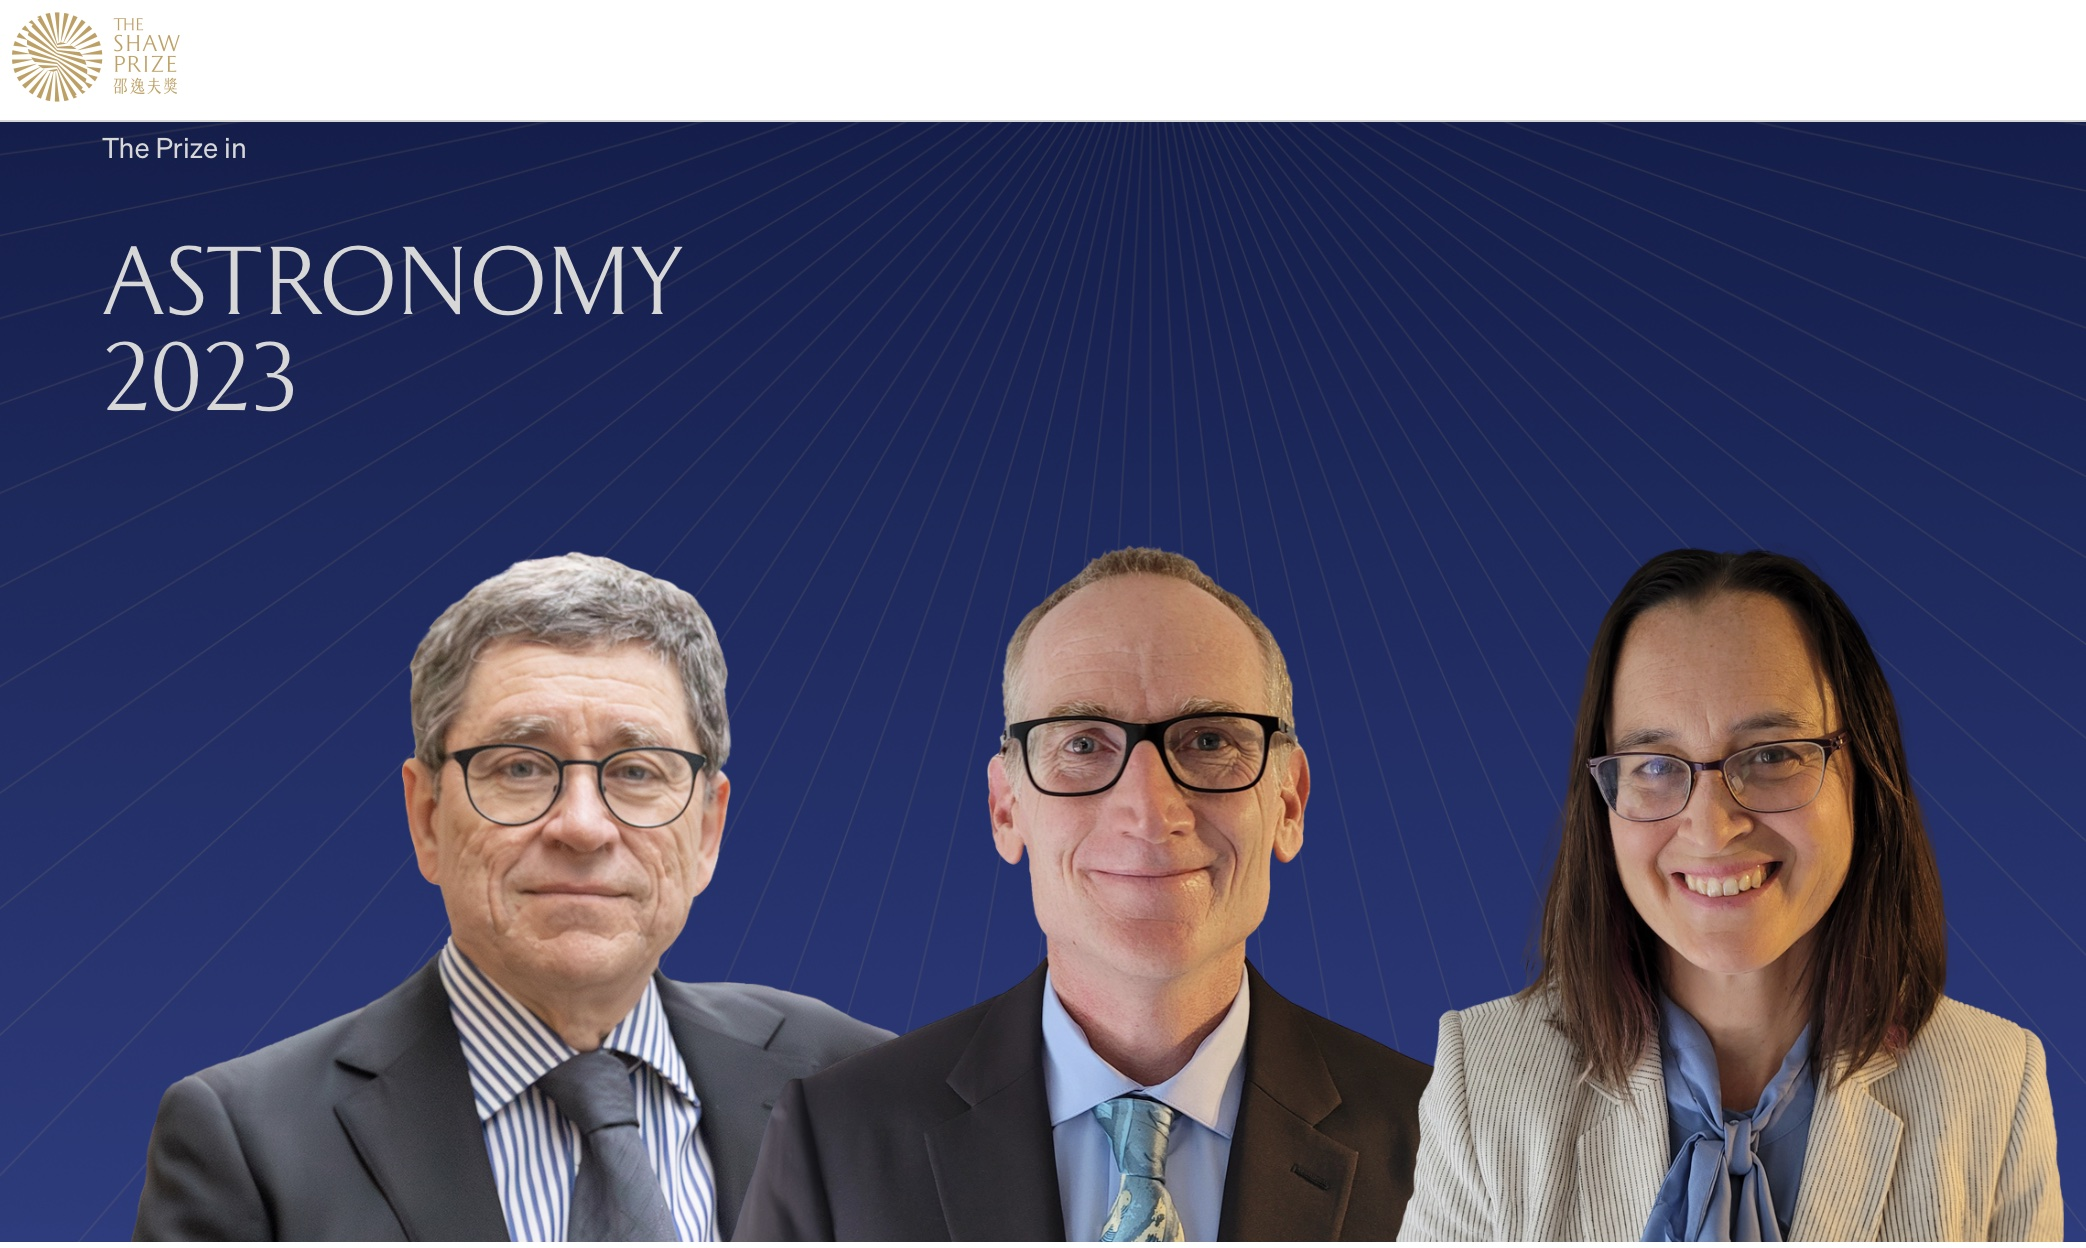
\includegraphics[width=4.5in]{Figures/shaw2023.jpg}
  }


  \frame{
    \frametitle{Fast Radio Bursts}
\small

The Shaw Prize in Astronomy 2023 is awarded in equal shares to {\bf Matthew
Bailes, Duncan Lorimer}, and {\bf Maura McLaughlin} the discovery of fast
radio bursts (FRBs).

FRBs are among the most extreme and mysterious phenomena in astronomy:
they are intense bursts of radio emission lasting only a few
thousandths of a second that contain as much energy as the Sun emits
over several days. The sources of the bursts are smaller than the
Earth but are as far away as distant galaxies. In a seminal research
paper written in 2007, Bailes, Lorimer, McLaughlin (with collaborators
Narkevic and Crawford) found the first FRB; deduced many of the
properties of its source, in particular its extreme distance, small
size, and enormous energy; estimated the cosmic rate of production of
FRBs; and highlighted their potential as cosmological probes.

  }


  \frame{
\vspace{-0.25in}
    \frametitle{FRB110523}
 

%\hspace{2.5in}
\includegraphics[width=2.5in]{Figures/scint110523.png}
\includegraphics[width=1.75in]{Figures/corr110523.png}

Masui++ 2015, Nature, 528, 523
  }



  \frame{
    \frametitle{Fast Radio Bursts}
    \begin{itemize}
      \item thousands detected, dozens localized
      \item generally highly polarized, complex RM/angle structure
      \item dozens of Nature papers
        \item Interference effects under multi-path propagation
        \item potential for diffraction limited measurements
        \item Kirchoff-Fresnel path integral
        \item effervescent images
        \item BURSTT
    \end{itemize}
  }

  \frame{
    \frametitle{Coherence}
    \begin{itemize}
        \item sensitive to ns time delay propagating for gigaparsecs
        \item corresponds to strain $h \ll 10^{-26}$: far exceeds LIGO
        \item highly elongated antenna pattern: sensitive to
          longitudinal modes          
    \end{itemize}
  }

  \frame{
    \frametitle{What are they?}
    \begin{itemize}
      \item mean luminosity: modest
      \item instantaneous intensity: $\sim 10^{40}$K
        \item beaming?
        \item pulsar analogs: crab beaming, companion plasma lensing,
          etc.  
          \item measured $\gamma \sim 10^4$, beaming correction $\sim 10^8$
        \item not seen in MW. Rare event, Short life span?
    \end{itemize}
  }


  \frame{

    \frametitle{TDE recyling?}
\begin{center}
\includegraphics[width=2.1in]{Figures/lipen.jpg}
\end{center}
  }




  \frame{
\vspace{-0.5in}
    \frametitle{New Observables}
    \begin{itemize}
    \item for coherent sources: FRBs, pulsars
    \item effervescent (complex) image allows time delay measurement (Jow+21)
    \item microlensing: instant time delay, planets (Jow+20)
    \item macrolensing: potentially nano-second delay -- universe
      expands!  Dark energy, etc (Wucknitz+21)
    \item dimensionless strain cm/Gigalightyears $h\sim \Delta t/t \sim 10^{-26}$:
      competitive with LIGO, etc
    \end{itemize}
  }


  \frame{
%\vspace{-0.25in}
    \frametitle{Macro lensing}
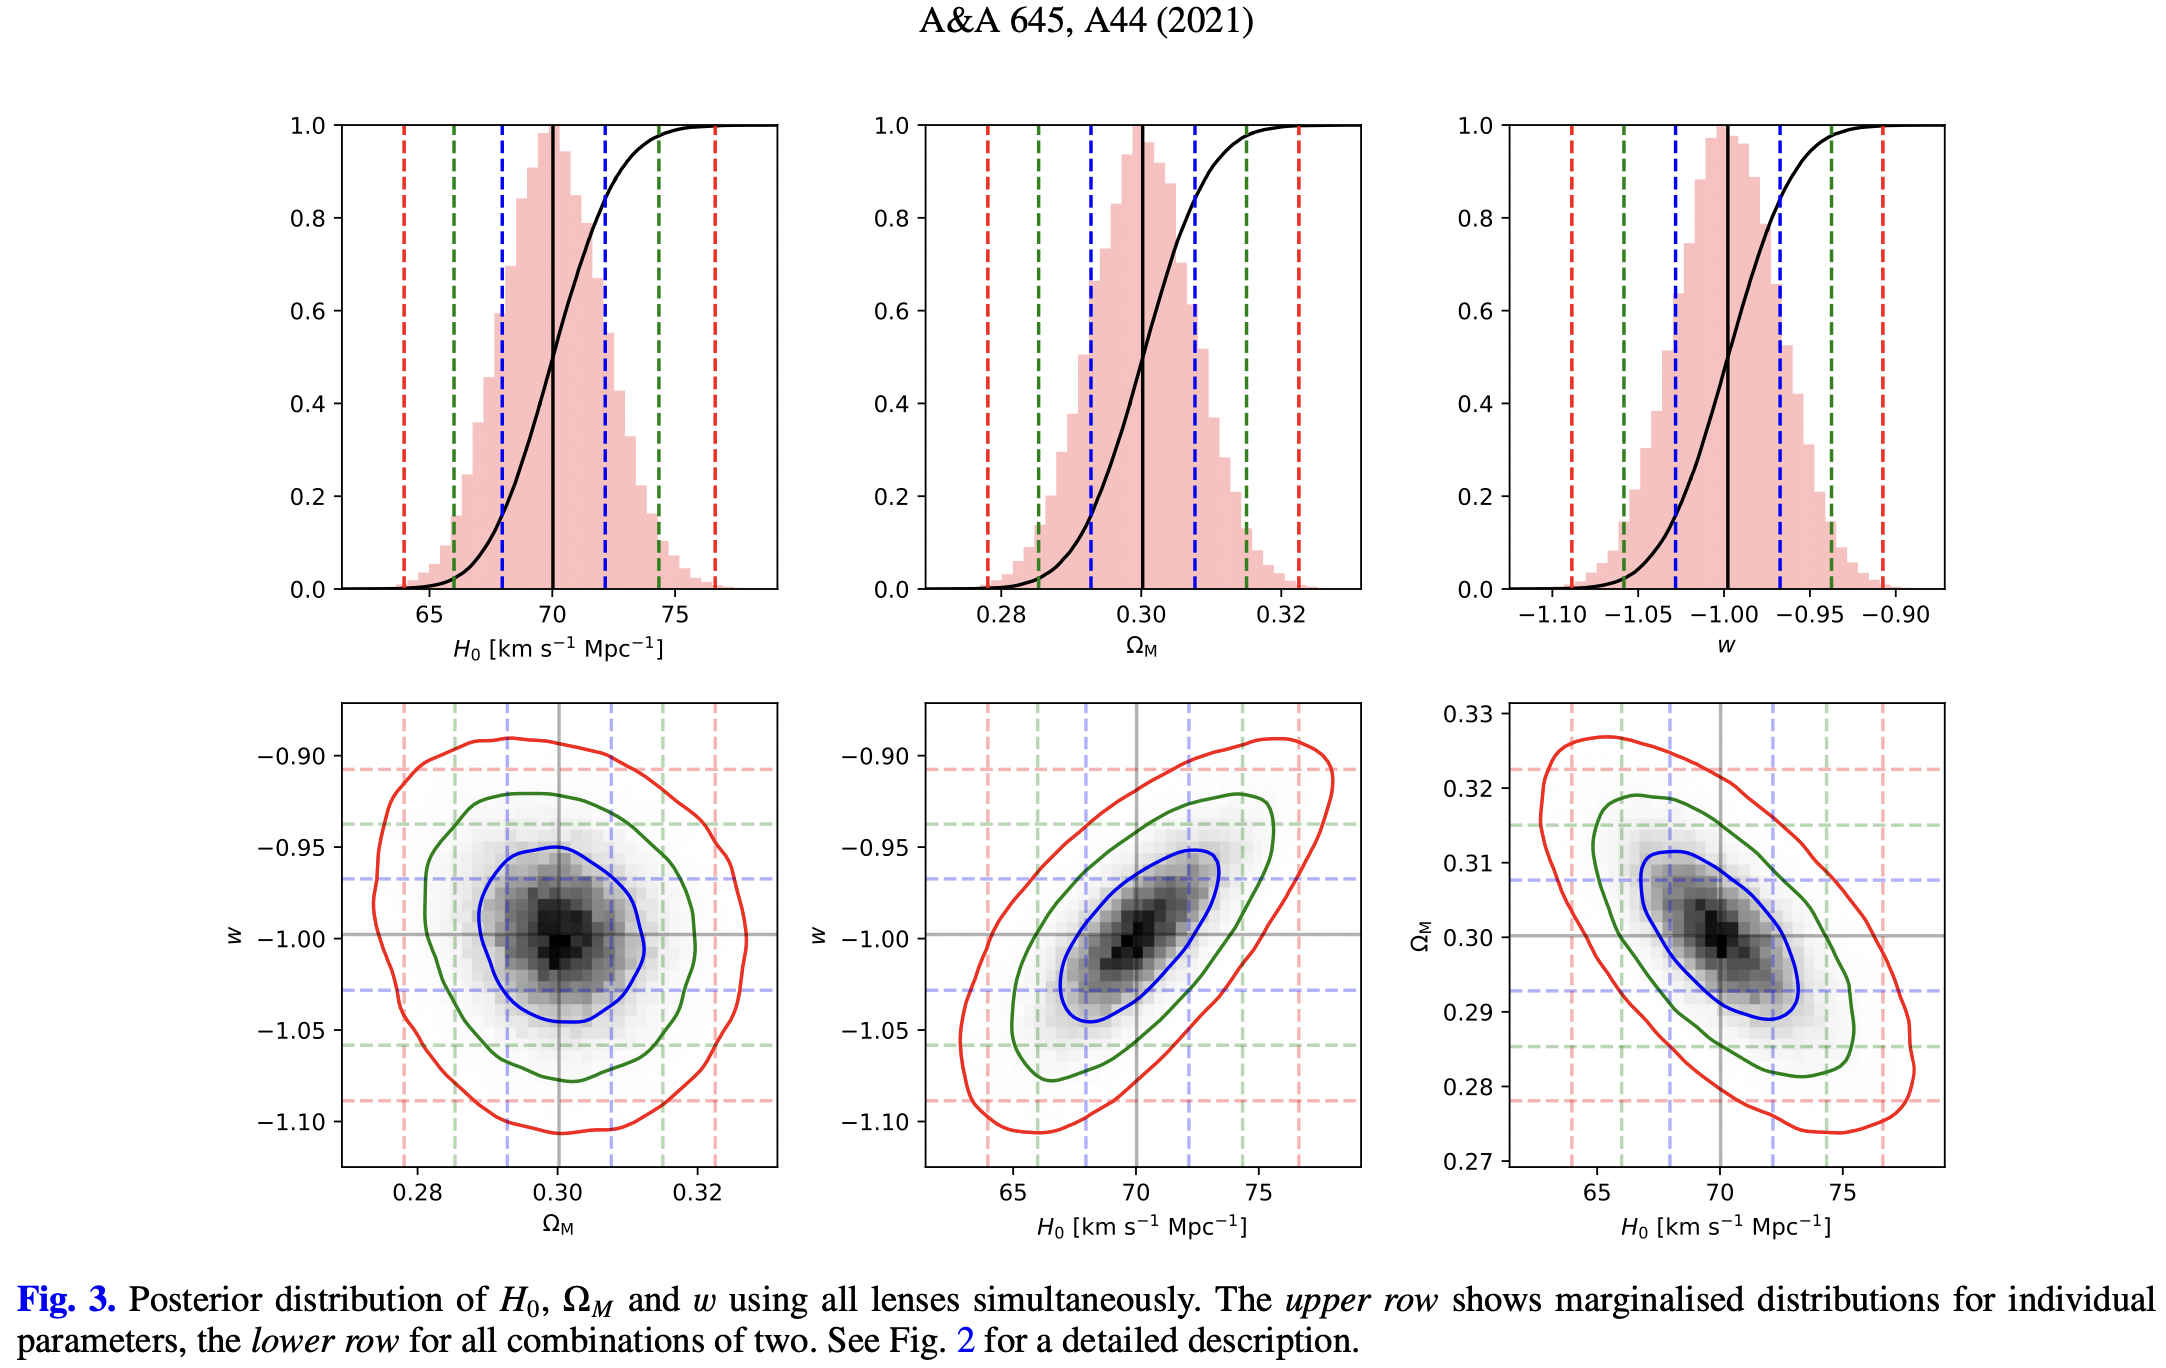
\includegraphics[width=4.5in]{Figures/wucknitz.png}

Wucknitz, Spitler, ULP 2021, A\&A, 645, A44
  }




  \frame{
\vspace{-0.5in}
    \frametitle{BURSTT}
    \begin{itemize}
    \item Bustling Universe Radio Survey Telescope in Taiwan
    \item instant wide field, VLBI localization
    \item nearby counterparts, multi-wavelength, multi-messenger
    \item repeat statistics
    \item bright sample for deep followup
    \end{itemize}
  }

  \frame{

    \frametitle{BURSTT}
\vspace{-0.25in}
\begin{center}
\hspace{-0.5in}
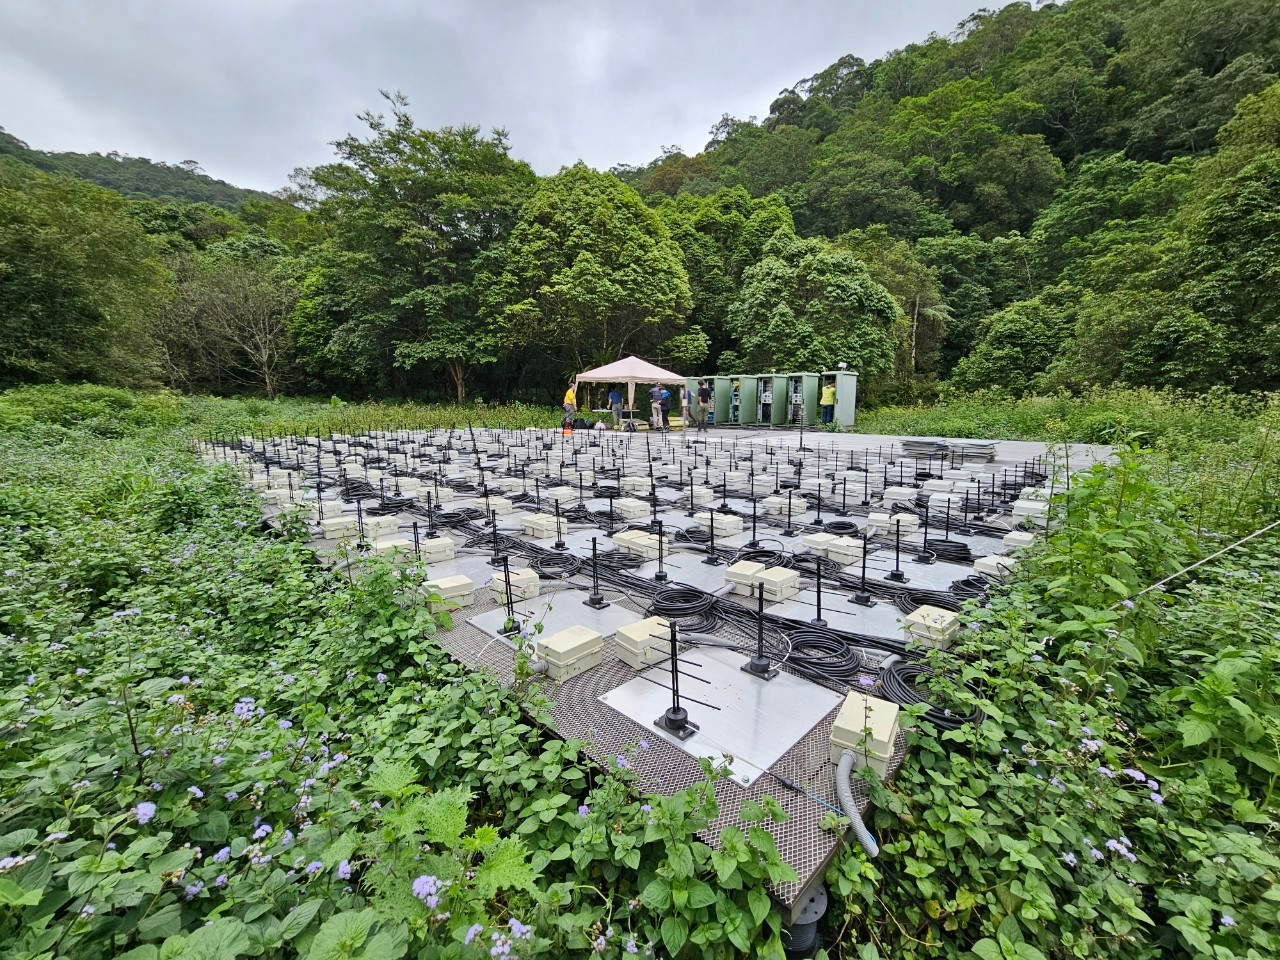
\includegraphics[width=4.9in]{Figures/burstt.jpg}
\end{center}
  }


  \frame{
    \frametitle{BURSTT network}
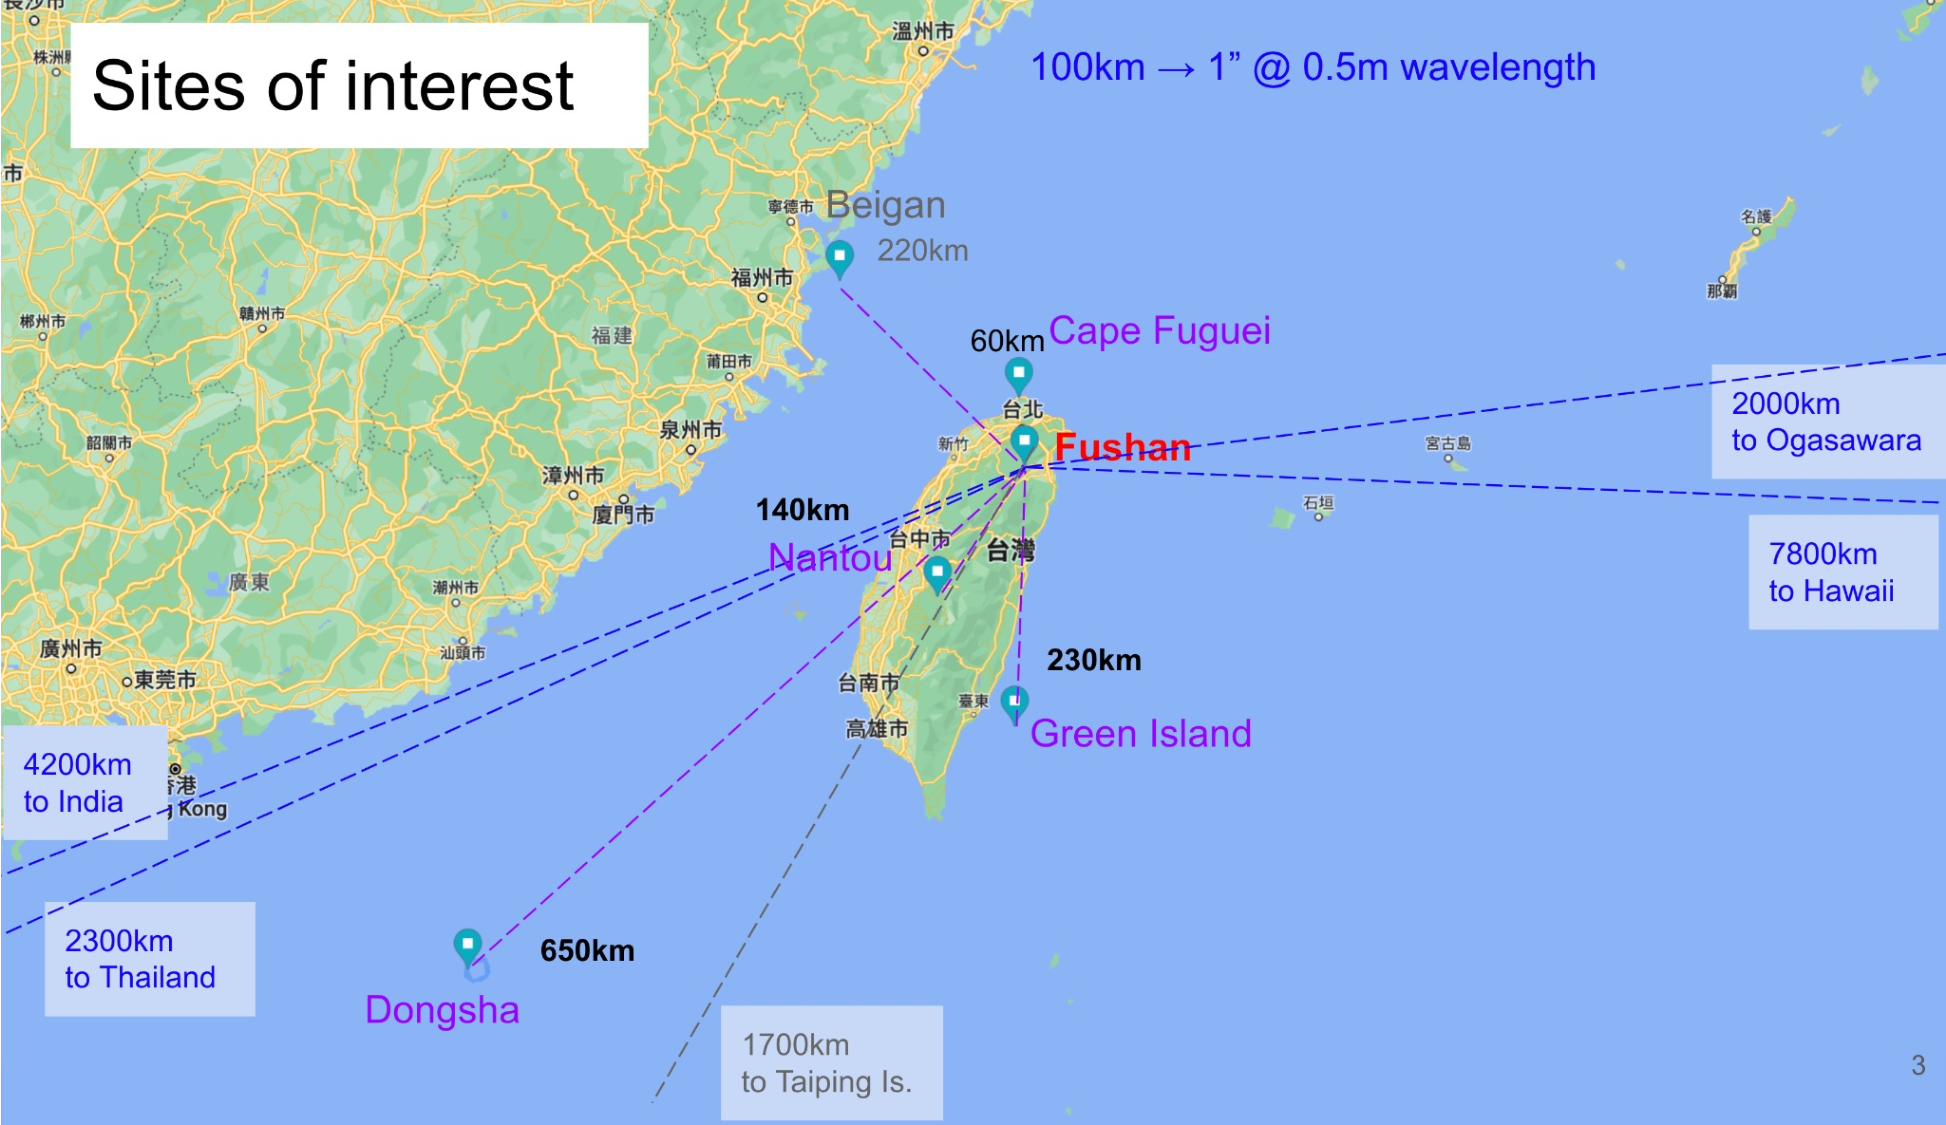
\includegraphics[width=4.5in]{Figures/bursttsites.pdf}
  }


  \frame{
    \frametitle{Outrigger stations}
\includegraphics[width=3.5in]{Figures/burstt-outrigger.jpg}
  }


  \frame{
%\vspace{-0.5in}
    \frametitle{Conclusions}
    \begin{itemize}
      \item FRB are unique coherent sources enabling unprecedented
        interference measurements
     \item wave optics changes nature of astrophysical observables: Coherent FRB/pulsar/GW      radiation one of the potentially most
      precise measurements in physics
      \item next generation FRB telescopes for cosmic mass and baryon inventory,
        possibly dark energy/acceleration
    \end{itemize}
  }

\end{document}
